\documentclass[11pt]{article}

\usepackage[letterpaper,margin=1in]{geometry}
\usepackage{amsmath,amssymb,mathtools}
\usepackage{booktabs}
\usepackage{longtable}
\usepackage{array}
\usepackage{xcolor}
\usepackage{fancyvrb}
\usepackage{microtype}
\usepackage{tikz}
\usetikzlibrary{arrows.meta,positioning,shapes.geometric,fit,calc}
\usepackage[hidelinks,colorlinks=true,linkcolor=blue!55!black,
            urlcolor=blue!55!black]{hyperref}

% --- shorthands -------------------------------------------------------------
\newcommand{\code}[1]{\texttt{\footnotesize #1}}
\newcommand{\eq}[1]{\textsf{#1}}                 % paper equation label
\newcommand{\chh}{\chi}
\newcommand{\lam}{\lambda}
\newcommand{\Phizero}{\Phi_{00}}
\newcommand{\Psizero}{\Psi_{0}}
\newcommand{\Dgrow}{D}
\newcommand{\Hcal}{\mathcal{H}}
\newcommand{\wjjj}[1]{\begin{pmatrix}#1\end{pmatrix}}
\DeclareMathOperator{\Real}{Re}

\setlength{\parindent}{0pt}
\setlength{\parskip}{0.5ex}
\setlength{\tabcolsep}{4pt}
\setlength{\emergencystretch}{3em}   % let TeX break \texttt-heavy prose lines
\sloppy

\title{\textbf{Equal-time Limber $\kappa_3$ vertex:\\ complete math flow (matter $P(k)\to\zeta$)}}
\author{\texttt{scripts/sachs\_sft/callables/kappa3\_vertex/equal\_time\_limber}}
\date{Traced from the canoes source (2026-06-02) and cross-checked against the STF\_lensing paper}

\begin{document}
\maketitle

\noindent
This note traces the \emph{entire production path} that turns the bare matter power
spectrum $P_\delta(k,z{=}0)$ into the equal-time third-cumulant table $\zeta_{XYZ}$
that the sft-wick non-local $K$-vertex consumes. Every computational step is paired
with (a)~the equation it implements, (b)~the exact \code{file:line} in code, and
(c)~the authoritative paper equation it corresponds to.

\medskip
\noindent\textbf{Symbols.}
$\chh$ comoving distance, $\lam$ affine projection parameter, $\ell$ multipole,
$\gamma$ angular separation, $\Phizero$/$\Psizero$ the two driving fields,
$H_0$ Hubble, $\Omega_m$, $\Dgrow$ linear growth, $A$ Poisson amplitude,
$\Hcal=$ conformal Hubble $\mathcal H$.

\smallskip
\noindent\textbf{Roots.}
Code \code{CAN = /Users/zzhang/projects/canoes/src/canoes};\quad
paper \code{PAP = .../STF\_lensing/sections}.

\tableofcontents

%======================================================================
\section{Pipeline at a glance}
%======================================================================
The build script
\code{build\_equal\_time\_limber\_table.py} (this folder) is only the conductor:
it passes arguments and sums two branches
(\code{build:133--151}).

\begin{center}
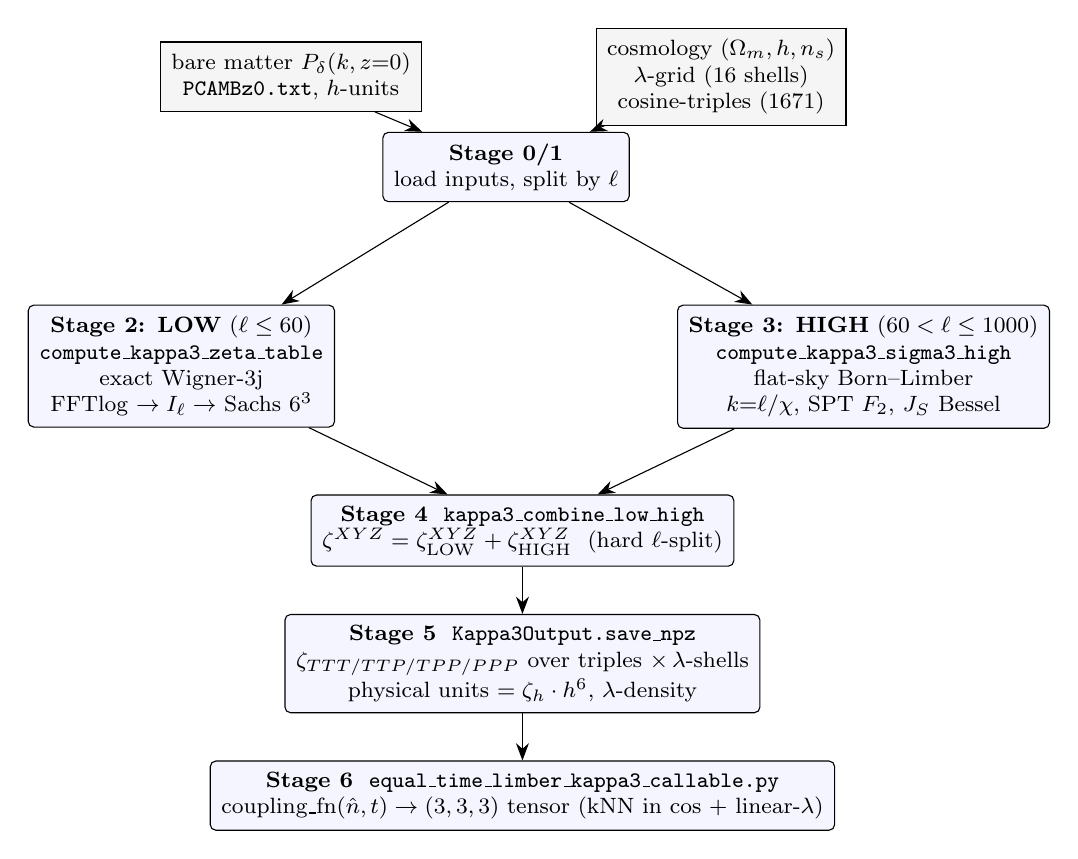
\begin{tikzpicture}[
  font=\footnotesize,
  box/.style={draw, rounded corners=2pt, align=center, inner sep=4pt,
              minimum height=8mm, fill=blue!4},
  io/.style={draw, align=center, inner sep=4pt, fill=gray!8},
  >={Stealth[length=2.2mm]}, node distance=6mm and 10mm,
]
\node[io] (pk) {bare matter $P_\delta(k,z{=}0)$\\ \code{PCAMBz0.txt}, $h$-units};
\node[io, right=22mm of pk] (cos) {cosmology $(\Omega_m,h,n_s)$\\
       $\lam$-grid (16 shells)\\ cosine-triples (1671)};
\node[box, below=7mm of $(pk)!0.5!(cos)$] (cond)
       {\textbf{Stage 0/1}\\ load inputs, split by $\ell$};
\node[box, below left=13mm and 6mm of cond] (low)
       {\textbf{Stage 2: LOW}\ ($\ell\le 60$)\\
        \code{compute\_kappa3\_zeta\_table}\\
        exact Wigner-3j\\ FFTlog $\to I_\ell\to$ Sachs $6^3$};
\node[box, below right=13mm and 6mm of cond] (high)
       {\textbf{Stage 3: HIGH}\ ($60<\ell\le 1000$)\\
        \code{compute\_kappa3\_sigma3\_high}\\
        flat-sky Born--Limber\\ $k{=}\ell/\chh$, SPT $F_2$, $J_S$ Bessel};
\node[box] (comb) at ($(low.south)!0.5!(high.south)+(0,-13mm)$)
       {\textbf{Stage 4}\ \ \code{kappa3\_combine\_low\_high}\\
        $\zeta^{XYZ}=\zeta_{\mathrm{LOW}}^{XYZ}+\zeta_{\mathrm{HIGH}}^{XYZ}$\ \ (hard $\ell$-split)};
\node[box, below=6mm of comb] (npz)
       {\textbf{Stage 5}\ \ \code{Kappa3Output.save\_npz}\\
        $\zeta_{TTT/TTP/TPP/PPP}$ over triples $\times\,\lam$-shells\\
        physical units $=\zeta_h\cdot h^6$, $\lam$-density};
\node[box, below=6mm of npz] (call)
       {\textbf{Stage 6}\ \ \code{equal\_time\_limber\_kappa3\_callable.py}\\
        $\mathrm{coupling\_fn}(\hat n,t)\to(3,3,3)$ tensor (kNN in $\cos$ + linear-$\lam$)};

\draw[->] (pk) -- (cond);
\draw[->] (cos) -- (cond);
\draw[->] (cond) -- (low);
\draw[->] (cond) -- (high);
\draw[->] (low) -- (comb);
\draw[->] (high) -- (comb);
\draw[->] (comb) -- (npz);
\draw[->] (npz) -- (call);
\end{tikzpicture}
\end{center}

%======================================================================
\section{Stage 0 --- Inputs}
%======================================================================
\subsection{Matter power spectrum (the single field-theory primitive)}
\begin{align}
&P_\delta(k,z{=}0)\ \text{from \code{PCAMBz0.txt}}\quad
   [\,k\ \text{in } h/\mathrm{Mpc},\ P\ \text{in } (\mathrm{Mpc}/h)^3\,]\notag\\
&\text{low-}k:\quad P(k)=P(k_{\min})\,(k/k_{\min})^{n_s},\qquad n_s=0.97\notag\\
&\text{high-}k:\ \text{raises};\qquad \text{in range: log--log linear interpolation.}
\end{align}
\textit{code:} \code{\_local\_cosmo\_pk.py:42--53} (feeds the bare matter $P_\delta$,
not $P_\Phi$); class \code{\_CambTablePk} \code{CAN/cosmo/pk.py:85--154}.\\
\textit{paper:} $P_\Phi(k;z{=}0)$ is named the single time-independent primitive
(\code{PAP/appendix.tex:496--500}); link $P_\delta(k)=[k^2/A(a{=}1)]^2\,P_\Phi(k)$ in
\eq{eq: appendix bphi tree} (\code{appendix.tex:608--614}).

\subsection{Cosmology}
\begin{equation}
\Omega_m=\frac{\Omega_c h^2+\Omega_b h^2}{h^2}
        =\frac{0.12029+0.02207}{0.6711^2}=0.3160919980475834,\quad h=0.6711,\ n_s=0.97.
\end{equation}
\textit{code:} \code{\_local\_cosmo\_pk.py:33--39}; defaults \code{CAN/cosmo/background.py:42--51}.

\subsection{Radial grid ($\lam$-shells) and angular grid (cosine-triples)}
$\lam$-shells: 16 nodes $396.6\ldots 2326.6$ Mpc ($z=0.1\ldots 5.7$), read from the L2 NPZ.
Triples $(\cos\gamma_{12},\cos\gamma_{23},\cos\gamma_{31})$ on a 15-node $\cos$-grid
($\cos=k/7$), triangle-filtered to 1671 realizable triples.\\
\textit{code:} $\lam$-grid \code{build:61--69}; triangle filter \code{build:72--81}.

%======================================================================
\section{Stage 2 --- LOW branch (exact Wigner-3j, $\ell\le 60$)}
%======================================================================
Entry \code{compute\_kappa3\_zeta\_table} \code{CAN/sachs/kappa3.py:3777}. The vertex
factorizes into a \emph{radial} stage (build $b_{\ell_1\ell_2\ell_3}(\lam)$) and an
\emph{angular} stage (Wigner-3j $\to\zeta$).

\subsection{FFTlog decomposition of $P_\delta$ ($N_{\max}=128$ Mellin modes)}
\begin{equation}
P_\delta(k)\approx\sum_n c_n\,k^{\nu_n},\qquad
\nu_n=\mathrm{bias}+\frac{2\pi i\,n}{N_{\max}\,\Delta\kappa},\quad
\mathrm{bias}=-1.6,\ N_{\max}=128 .
\end{equation}
$N_{\max}$ is the number of FFTlog $k$-samples (not a Bessel order, not the bandlimit
$\ell_{\max}$). \textit{code:} \code{CAN/nuell/transfer/fftlog.py:43--131};
half-spectrum build \code{kappa3.py:458--466}.

\subsection{Radial double-Bessel transform (the $I_\ell$ kernel)}
\begin{align}
I_\ell(\nu,t)&=4\pi\int_0^\infty dv\,v^{\nu-1}\,j_\ell(v)\,j_\ell(vt),
   \qquad\text{(ASZ-2017 Mellin integral)}\\
P_\ell(r;\chh)&=\sum_n c_n\,\chh^{-\nu_n}\,\frac{I_\ell(\nu_n+\mathrm{shift},\,r/\chh)}{4\pi}
   \quad\text{(power-law ``PL'' leg)},
\end{align}
plus a closure leg $S^{\mathrm{spec}}_\ell(r;\chh)$ ($\delta^2$ SPT leg, $\Gamma$-regularized).\\
\textit{code:} $I_\ell$ \code{kernels/il.py:1--6,1288}; PL leg \code{\_bl\_jax.py:679--698};
spec leg \code{\_bl\_jax.py:700--717}.\quad
\textit{paper:} per-leg $\Delta_\ell^X(k;\lam)$ is \eq{eq: appendix delta ell}
(\code{appendix.tex:562--568}); per-leg kernel $M'_\ell$ is \eq{eq: appendix Mprime}
(\code{appendix.tex:653--659}).

\subsection{Tree-level SPT layout $+$ the Sachs $6\times6\times6$ basis contraction}
\begin{equation}
\begin{aligned}
b_{\ell_1\ell_2\ell_3}(\lam)=\Bigl(\tfrac{2}{\pi}\Bigr)^{3}
   &\sum_{k,l,m\in\mathrm{basis}(6)}(C_a\!\cdot\!M)_k\,(C_b\!\cdot\!M)_l\,(C_c\!\cdot\!M)_m\\[-2pt]
   &\times\sum_{\substack{3\ \mathrm{cyc}\\ \mathrm{spec}}}\ \sum_{6\ F_2\ \mathrm{mono}}
     \mathrm{coeff}\int_0^\infty\! dr\,r^2\,
     S^{\mathrm{spec}}_{\ell_c}(r;\chh)\,P_{\ell_a}(r;\chh)\,P_{\ell_b}(r;\chh)\
     \times\Delta_{\mathrm{tri}}(\ell_1\ell_2\ell_3).
\end{aligned}
\label{eq:bllow}
\end{equation}
The $18=(3\ \text{cyclic spectator})\times(6\ F_2\ \text{monomials})$ terms encode the
SPT tree matter bispectrum $B_\delta=2F_2PP+\mathrm{cyc}$; $(C_a,C_b,C_c)$ are the per-leg
Sachs CoefVecs (\S\ref{sec:coef}), $M$ the lightcone derivative basis (\S\ref{sec:M}).\\
\textit{code:} $r$-integral leaf \code{\_bl\_jax.py:914--917}; $6^3$ contraction
\code{\_bl\_jax.py:1081--1087}; SPT monomials \code{\_phi\_accumulator.py:49--69}.\quad
\textit{paper:} this is exactly \eq{eq: appendix b prime} (\code{appendix.tex:667--675}),
$B'^{XYZ}_{LL\ell_3}=(2/\pi)^3\!\int dr\,r^2\sum_{t=0}^{17}c_t\,M'^{\mathrm{spec}}_\ell M'^{\mathrm{PL}}_\ell M'^{\mathrm{PL}}_\ell$.

\subsection{The cosmology prefactor stack (applied per $\lam$-shell)}
\label{sec:prefac}
The dimensionless [angular $\times$ SPT-shape] integral is multiplied by, in order:
\begin{center}
\renewcommand{\arraystretch}{1.5}
\scriptsize
\begin{tabular}{@{}c l >{\raggedright\arraybackslash}p{5.9cm} >{\raggedright\arraybackslash}p{4.1cm}@{}}
\toprule
\# & factor & equation & code \\
\midrule
i  & Poisson$^3$ & $A(a)^3=\bigl[-\tfrac32 H_0^2\Omega_m(1{+}z)\bigr]^3$,\ \ $H_0=100/c$ ($h$-indep.) & \code{kappa3.py:85,4222--4224}; cubed \code{:4268--4269} \\
ii & Sachs geometric & $\bigl((1{+}z)^P\bigr)^3=(1{+}z)^{12}$,\ \ $P=\textsf{SACHS\_GEOMETRIC\_POWER}=4$ & \code{kappa3.py:499}; \code{sachs\_driver.py:97} \\
iii& per-leg $M$ & $s_X=C_X\!\cdot\!M$,\ $M[0]{=}\Dgrow(1{+}z),\ M[1]{=}-\partial_\chh[\Dgrow(1{+}z)],\ M[2]{=}\partial_\chh^2[\cdots]$ & \code{kappa3.py:482--512}; \code{lightcone.py:342--350} \\
iv & spectator growth & $\times\,\Dgrow(z)=M[0]/(1{+}z)$\ \ (promotes $\Dgrow^3\!\to\!\Dgrow^4$) & \code{kappa3.py:4495--4506} \\
v  & radial measure & $\lam$-density $\Rightarrow\ \times 1$\ \ (\emph{no} $(d\chh/d\lam)$ Jacobian) & \code{kappa3.py:1761--1805,4508--4520} \\
vi & units & physical $\Rightarrow\ \zeta=h^6\zeta_h$,\ $\chh\!\to\!\chh/h$,\ $\lam\!\to\!\lam/h$ & \code{kappa3.py:4522--4530} \\
\bottomrule
\end{tabular}
\end{center}
\textit{paper:} per-leg $A(a)=-\tfrac32 H_0^2\Omega_m/a$ and per-leg $(1{+}z)^4$ Sachs weight,
\code{appendix.tex:603--604,536--543}; measure $d\lam=a^2(\chh)\,d\chh$ in
\eq{eq: cumulant 2 measure change} (\code{cosmology.tex:979--988}); $\bar D=a\chh$ in
\eq{eq: D equals a chi} (\code{appendix.tex:286--289}).

\begin{quote}\small\color{red!60!black}
\textbf{Warning.} The redshift scaling is \emph{not} a clean power (see \S\ref{sec:zscaling}).
The growth is clean ($\Dgrow^4$), but the $(1{+}z)$ content is heterogeneous because
\textsf{COEFS\_PHI00} contracts $M[0],M[1],M[2]$ together with the $\Hcal^2/\Hcal'/L^2\chh^{-2}$
operator terms.
\end{quote}

\subsection{The lightcone derivative basis $M[0..2]$}
\label{sec:M}
\begin{equation}
M[0]=\Dgrow(z)(1{+}z)=\Dgrow/a,\quad
M[1]=-\frac{d}{d\chh}\bigl[\Dgrow(1{+}z)\bigr],\quad
M[2]=\frac{d^2}{d\chh^2}\bigl[\Dgrow(1{+}z)\bigr],
\end{equation}
with $\Hcal=E(z)/\bigl[(1{+}z)(c/100)\bigr]$, $E(z)=\sqrt{\Omega_m(1{+}z)^3+1-\Omega_m}$.
\textit{code:} \code{CAN/cosmo/lightcone.py:328--329,342--350}.

\subsection{The per-leg Sachs CoefVecs (what makes $T$ vs $P$)}
\label{sec:coef}
\begin{align}
\textsf{COEFS\_PHI00}&=\Bigl(\tfrac{L^2}{\chh^2}+2\Hcal^2-2\Hcal',\ -\tfrac{2}{\chh}+2\Hcal,\ -1,\ 0,\ -1,\ 2\Bigr) && (T=\Phizero,\ \text{spin }0),\\
\textsf{COEFS\_PSI0}&=\Bigl(-\tfrac{\sqrt{L^2(L^2-2)}}{\chh^2},\ 0,0,0,0,0\Bigr) && (P=\Psizero,\ \text{spin }2),
\end{align}
with $L^2=\ell(\ell+1)$. A leg's operator value is
$g_{\mathrm{leg}}(\ell,\chh)=\sum_{k=0}^{5}\textsf{COEFS}[k]\,M[a_k]$, the gather
$a_k=[0,0,0,1,2,1]$.\quad \textit{code:} \code{CAN/nuell/transfer/sachs\_driver.py:74--90};
gather \code{kappa3.py:482--484}; $L^2=\ell(\ell+1)$ \code{basis.py:45--52,111--120}.

\subsection{Angular stage --- exact Wigner-3j $\to\zeta$}
\label{sec:angular}
For each cosine-triple with channel spins $(s_1,s_2,s_3)$:
\begin{equation}
\begin{aligned}
\zeta_{\mathrm{LOW}}^{XYZ}(\gamma_{12},\gamma_{23},\gamma_{31};\lam)
 =\Dgrow(z)\!\!\sum_{\ell_1\ell_2\ell_3\le 60}\!\! b_{\ell_1\ell_2\ell_3}(\lam)\,
   &h\,\wjjj{\ell_1&\ell_2&\ell_3\\0&0&0}\sqrt{\tfrac{2\ell_1+1}{4\pi}}(-1)^{s_1}\\[-2pt]
 \times\sum_{m_2}\ &\wjjj{\ell_1&\ell_2&\ell_3\\-s_1&m_2&s_1-m_2}
   {}_{s_2}Y_{\ell_2 m_2}(\gamma_{12},0)\ {}_{s_3}Y_{\ell_3,\,s_1-m_2}(\gamma_{31},\varphi_3),
\end{aligned}
\label{eq:zetalow}
\end{equation}
with $h=\sqrt{(2\ell_1+1)(2\ell_2+1)(2\ell_3+1)/4\pi}$. Two Wigner-3j symbols appear:
the parity/triangle anchor $(\ell_1\ell_2\ell_3;0,0,0)$ (kept for \emph{all} four channels)
and the $m$-resolved $(\ell_1\ell_2\ell_3;-s_1,m_2,s_1{-}m_2)$. Angular separations enter
through ${}_sY$ with $\theta=\arccos\cos\gamma$; the leading $\Dgrow(z)$ is the spectator
growth.\\
\textit{code:} scalar (TTT) \code{three\_pt.py:516--645}; spin-weighted
\code{\_spin\_aware\_three\_pt.py:15--289}; GEMV \code{\_jax\_kernels.py:1012--1032}.\quad
\textit{paper:} this is \eq{eq: appendix zeta squeezed} (\code{appendix.tex:684--704}),
\begin{gather}
\zeta_{XYZ}(\gamma)=\!\!\sum_{\substack{L,\ell_3\\ 2L+\ell_3\ \mathrm{even},\,\ell_3\le 2L}}\!\!
   \mathcal{G}(L,L,\ell_3)\,P_{\ell_3}(\cos\gamma)\,B'^{XYZ}_{LL\ell_3},\notag\\
\mathcal{G}(L,L,\ell_3)=\frac{(2L{+}1)^2(2\ell_3{+}1)}{(4\pi)^2}\bigl[w_{3j}(L,L,\ell_3;0,0,0)\bigr]^2 .
\end{gather}
The paper writes the squeezed $(L,L,\ell_3)$ specialization (Legendre $P_{\ell_3}(\cos\gamma)$,
two rays coincident); the code's general $m$-sum reduces to it for that configuration.

%======================================================================
\section{Stage 3 --- HIGH branch (flat-sky Born--Limber, $60<\ell\le 1000$)}
%======================================================================
Entry \code{compute\_kappa3\_sigma3\_high} \code{CAN/sachs/kappa3.py:3406--3684}.

\subsection{Flat-sky Limber collapse ($k=\ell/\chh$, single shell)}
\begin{gather}
u=|\boldsymbol\ell_2|,\quad v=|\boldsymbol\ell_3|,\quad \varphi=\angle(\boldsymbol\ell_2,\boldsymbol\ell_3),\quad
w=|\boldsymbol\ell_1|=\sqrt{u^2+v^2+2uv\cos\varphi},\notag\\
k_i=\frac{\ell_i}{\chh(\lam)}\ \ (\text{equal-}\chh\ \text{Limber}),\qquad \text{radial kernel}=\frac{1}{\chh^4}.
\end{gather}
(equal-$\chh$ Limber, no factor of $a$; the $1/\chh^4$ is three $1/\chh^2$ collapsed by two
equal-$\chh$ $\delta$'s.) \textit{code:} quadrature \code{kappa3.py:1608--1649}
($n_\ell{=}96$, $n_\varphi{=}64$); $k=\ell/\chh$ \code{:3570--3572}; $1/\chh^4$ \code{:3585}.

\subsection{Tree-level SPT matter bispectrum ($F_2$ kernel)}
\begin{align}
B_\delta(k_1,k_2,k_3)&=2\bigl[F_2(k_1,k_2)P_1P_2+F_2(k_1,k_3)P_1P_3+F_2(k_2,k_3)P_2P_3\bigr],\\
F_2(k_a,k_b)&=\frac57+\frac12\,\mu\Bigl(\frac{k_a}{k_b}+\frac{k_b}{k_a}\Bigr)+\frac27\mu^2,
   \quad \mu=\cos(k_a,k_b),\quad P_i=P_\delta(k_i,z{=}0).
\end{align}
\textit{code:} $F_2$ \code{kappa3.py:1690--1702}; $B$ assembly \code{:3573--3579}; internal
cosines from the closed $\ell$-triangle \code{:3530--3540}.\quad \textit{paper:} same SPT tree
in \eq{eq: appendix bphi tree} (\code{appendix.tex:608--614}).

\subsection{Cosmology factors (HIGH mirror of \S\ref{sec:prefac})}
\begin{equation}
\times\,\Dgrow(z)^4\ \ (B_\delta\propto PP\propto \Dgrow^4),\qquad
R_{\mathrm{channel}}=\prod_{\mathrm{legs}}(\pm)\,A(a)(1{+}z)^4,\qquad
\text{prefactor }\frac{1}{(2\pi)^4},
\end{equation}
$A(a)=-\tfrac32\Omega_m H_0^2(1{+}z)$; sign $+$ for $\Phizero$ ($T$), $-$ for $\Psizero$ ($P$).
\textit{code:} growth$^4$ \code{:3580--3583}; $A(a)$ \code{:3498--3500}; response product
\code{:1669--1687}, applied \code{:3589--3594}; $1/(2\pi)^4$ \code{:3541}.

\subsection{Spin via the analytic orientation (Bessel) integral}
\begin{equation}
\theta_{ij}=\arccos\cos\gamma_{ij},\quad
Q=u\,r_2+v\,e^{-i\varphi}r_3,\quad S=s_1+s_2+s_3,
\end{equation}
\begin{equation}
\alpha_{\mathrm{channel}}=\Real\!\Bigl[2\pi\,i^{S}e^{iS\arg Q}J_S(|Q|)\,
   e^{i(s_1\arg\boldsymbol\ell_1+s_3\varphi)}\Bigr]\quad
   \bigl(S{=}0\Rightarrow\alpha=2\pi J_0(|Q|)\bigr),
\end{equation}
with $r_2=\theta_{12}$, $r_3=x_3+iy_3$ (law of cosines). Spins:
TTT $(0,0,0)$, TTP $(0,0,2)$, TPP $(0,2,2)$, PPP $(2,2,2)$; all four nonzero in HIGH.
\textit{code:} vertices \code{kappa3.py:1705--1717}; $\alpha$-kernel \code{:1720--1758};
spins \code{:1664--1666}.

\subsection{HIGH assembled}
\begin{equation}
\begin{aligned}
\zeta_{\mathrm{HIGH}}^{XYZ}(\text{triple},\lam)=
\frac{1}{(2\pi)^4}\frac{\Dgrow^4}{\chh^4}\,R_{\mathrm{channel}}
\int du\,dv\,d\varphi\ (uv\,w_\ell w_\ell w_\varphi)\,B_\delta\,\alpha_{\mathrm{channel}},\\[2pt]
\text{integration region: }\ \ell_{\mathrm{cut}}<\max(\ell_1,\ell_2,\ell_3)\le\ell_{\mathrm{hi}}.
\end{aligned}
\end{equation}
\textit{code:} radial base \code{:3585}; weighted$\times\alpha$ sum \code{:3595--3596};
HIGH window \code{:3515--3518}.

%======================================================================
\section{Stage 4 --- Combine LOW $+$ HIGH}
%======================================================================
\begin{equation}
\zeta^{XYZ}(\text{triple},\lam)=\zeta_{\mathrm{LOW}}^{XYZ}(\text{triple},\lam)
 +\zeta_{\mathrm{HIGH}}^{XYZ}(\text{triple},\lam).
\end{equation}
A plain elementwise array sum on the \emph{identical} (cosine-triple, $\lam$) grid.
Hard split at $\ell_{\mathrm{cut}}$, no tapering: LOW does exact 3j for $\ell\le\ell_{\mathrm{cut}}$,
HIGH does flat-sky for $\max\ell\in(\ell_{\mathrm{cut}},\ell_{\mathrm{hi}}]$; the boundary
$\max\ell=\ell_{\mathrm{cut}}$ is in LOW only. Grid/units/measure compatibility is asserted
before the add; \texttt{cosmo\_meta} is merged.\quad
\textit{code:} \code{kappa3\_combine\_low\_high} \code{kappa3.py:3710--3774} (sum \code{:3766--3771},
grid checks \code{:3741--3742}).

%======================================================================
\section{Stage 5 --- Output table}
%======================================================================
\code{Kappa3Output} holds \texttt{cosine\_triples}$(M,3)$, \texttt{lambda\_shells\_Mpc},
\texttt{chi\_shells\_Mpc}, \texttt{z\_shells}, \texttt{zeta\_TTT/TTP/TPP/PPP}$(M,N_\lam)$,
\texttt{ell\_max}, \texttt{cosmo\_meta}. \code{save\_npz} writes them with
\emph{physical} units ($\lam,\chh$ in Mpc; $\zeta=h^6\zeta_h$) and \emph{$\lam$-density}
measure (no Jacobian).\quad \textit{code:} dataclass \code{kappa3.py:164--237};
\code{save\_npz} \code{:187--206}. The build then overwrites the metadata block
(\code{build:152--170}).

%======================================================================
\section{Stage 6 --- Callable consumption (what sft-wick sees)}
%======================================================================
\begin{gather}
\cos\gamma_{ij}=\hat n_i\!\cdot\!\hat n_j\ \xrightarrow{\text{sort desc}}\
\text{cKDTree query }(k{=}4\ \text{inverse-distance}),\qquad
\lam_{\mathrm{mean}}=\overline{t},\notag\\
\zeta_{\mathrm{ch}}=\frac{\sum_k w_k\,\zeta_{\mathrm{ch}}[\text{node}_k,\lam]}{\sum_k w_k}.
\end{gather}
The $(3,3,3)$ tensor places
$\zeta_{TTT}$ at $[0,0,0]$, $\zeta_{TTP}$ at the $\{0,0,1\}$ perms, $\zeta_{TPP}$ at $\{0,1,1\}$,
$\zeta_{PPP}$ at $[1,1,1]$; all index-2 (B-mode) entries are zero. Because
\texttt{already\_R\_contracted}$=$False, sft-wick applies the response $R$ itself (this table is the
bare vertex $K$).\quad \textit{code:} \code{callable.py:129--228}. See the \texttt{slices/} figures:
a contact spike at the collapsed apex $\cos=(1,1,1)$ $\sim$100$\times$ above a flat
wide-separation plateau, growing toward high $z$.

%======================================================================
\section{Redshift scaling of $\zeta$ (the honest statement)}
\label{sec:zscaling}
%======================================================================
$\zeta_{TTT}(\mathrm{apex},z)$ does \textbf{not} factor as a clean
$(1{+}z)^P\,\Dgrow^Q\times[\text{$z$-independent shape}]$.
\begin{itemize}
\item \textbf{Growth is clean: $Q=4$.} Three per-leg $M$-factors (each linear in $\Dgrow$)
  $\times$ one spectator $\Dgrow$. No extra $\Dgrow$ hides (the $\chh$-derivatives in
  $M[1],M[2]$ differentiate the \emph{shape}, not the amplitude). Metadata
  \textsf{growth\_scaling="D\textasciicircum 4"} is correct.
\item \textbf{$(1{+}z)$ is not clean.} Explicit factors give $(1{+}z)^{15}=(1{+}z)^{12}$
  [\S\ref{sec:prefac}\,ii] $\times(1{+}z)^3$ [Poisson cube, \S\ref{sec:prefac}\,i]. But
  $\sum_k\textsf{COEFS\_PHI00}[k]\,M[a_k]$ mixes $M[0]=\Dgrow(1{+}z)$ with $M[1],M[2]$
  ($\chh$-derivatives carrying $\Hcal$-content) and the $2\Hcal^2-2\Hcal'$, $L^2/\chh^2$
  terms in one slot. $\Hcal=E(z)/[(1{+}z)(c/100)]$ is not a power of $(1{+}z)$, so the exact
  exponent is ill-defined.
\item \textbf{Leading-term scaling} (keep only the ID$\cdot M[0]$ $L^2/\chh^2$ piece,
  dominant at $\ell\gtrsim$ a few):
\begin{equation}
\zeta_{TTT}(\mathrm{apex},z)\ \approx\
\Bigl[-\tfrac32 H_0^2\Omega_m\Bigr]^3 (1{+}z)^{15}\,\Dgrow(z)^4\,\chh^{-6}
\prod_i \ell_i(\ell_i+1)\ \cdot\ [\text{Wigner-3j}]\cdot\Bigl[\text{SPT}\!\int r^2dr\ \text{shape}\Bigr].
\end{equation}
\end{itemize}
This explains the slices: $\zeta$ grows steeply toward high $z$ (the $(1{+}z)^{15}\Dgrow^4$
front factor) and is sharply peaked at the collapsed apex.

%======================================================================
\section{Review --- production step $\leftrightarrow$ equation completeness}
%======================================================================
Every step in the production path, with its equation and a verdict on whether an equation is
attached.

\renewcommand{\arraystretch}{1.3}
\scriptsize
\begin{longtable}{@{}l >{\raggedright\arraybackslash}p{2.5cm} >{\raggedright\arraybackslash}p{4.8cm} >{\raggedright\arraybackslash}p{2.7cm} c@{}}
\toprule
step & action & code (\code{file:line}) & paper & ok\\
\midrule
\endfirsthead
\toprule
step & action & code & paper & ok\\
\midrule
\endhead
\bottomrule
\endfoot
S0.1 & load matter $P_\delta$ & \code{\_local\_cosmo\_pk.py:42--53}; \code{pk.py:85--154} & \eq{appendix.tex:496--500,608--614} & \checkmark\\
S0.2 & cosmology / grids & \code{build:61--81} & --- & \checkmark\\
S2.1 & FFTlog of $P_\delta$ & \code{fftlog.py:43--131} & (numeric) & \checkmark\\
S2.2 & double-Bessel $I_\ell$ & \code{il.py:1--6}; \code{\_bl\_jax.py:679--717} & \eq{delta ell}, \eq{Mprime} & \checkmark\\
S2.3 & SPT 18-term $+$ $6^3$ contraction & \code{\_bl\_jax.py:914--1087}; \code{\_phi\_accumulator.py:49--69} & \textbf{\eq{b prime}} & \checkmark\\
S2.4i & Poisson $A(a)^3$ & \code{kappa3.py:4222--4224,4269} & \eq{cosmology.tex:405--407}; \eq{appendix:603--604} & \checkmark$^{R1}$\\
S2.4ii & $(1{+}z)^{12}$ Sachs & \code{kappa3.py:499}; \code{sachs\_driver.py:97} & \eq{appendix:536--543} & \checkmark\\
S2.4iii & per-leg $M$ & \code{kappa3.py:482--512}; \code{lightcone.py:342--350} & \eq{Mprime} & \checkmark\\
S2.4iv & spectator $\Dgrow$ ($\to\Dgrow^4$) & \code{kappa3.py:4495--4506} & (code conv.) & \checkmark$^{R3}$\\
S2.4v & $\lam$-density ($\times1$) & \code{kappa3.py:1761--1805} & \eq{measure}; \eq{D=a$\chi$} & \checkmark\\
S2.4vi & $h^6$ units & \code{kappa3.py:4522--4530} & ($h$-bookkeeping) & \checkmark\\
S2.7 & exact Wigner-3j angular & \code{three\_pt.py:516--645}; \code{\_spin\_aware\_three\_pt.py:15--289} & \textbf{\eq{zeta squeezed}}$+\mathcal{G}$ & \checkmark$^{R2}$\\
S3.1 & flat-sky Limber $k{=}\ell/\chh$, $1/\chh^4$ & \code{kappa3.py:3570--3585, 1608--1649} & (Limber) & \checkmark\\
S3.2 & SPT $F_2$ matter bispectrum & \code{kappa3.py:1690--1702, 3573--3579} & \eq{bphi tree} & \checkmark\\
S3.3 & HIGH cosmology factors & \code{kappa3.py:3498--3500, 3580--3594, 1669--1687} & \eq{appendix:603--604} & \checkmark\\
S3.4 & spin Bessel orientation $J_S$ & \code{kappa3.py:1705--1758} & (flat-sky 3PCF) & \checkmark\\
S4 & LOW$+$HIGH sum & \code{kappa3.py:3710--3774} & (numerical $\ell$-split) & \checkmark\\
S5 & NPZ save (units, measure) & \code{kappa3.py:164--206} & --- & \checkmark\\
S6 & callable $\to(3,3,3)$ & \code{callable.py:129--228} & sft-wick contract & \checkmark\\
\end{longtable}

\normalsize
\textbf{Verdict:} every production step has a corresponding equation. Three points are
code$\leftrightarrow$paper \emph{conventions to keep on the radar} (not gaps):

\begin{description}
\item[R1 --- Poisson sign.] \code{cosmology.tex:405--407} writes $\Phizero=+A\delta$ with
  $A>0$; the appendix and the code use $A(a)=-\tfrac32 H_0^2\Omega_m/a$ ($A<0$). Because $A$
  enters cubed (odd power), the sign reaches $\zeta$. Code is consistent with the appendix; the
  main-text caption sign differs. A one-line paper reconciliation, not a code change.
\item[R2 --- spin-2 Wigner-3j.] Both code and paper keep the \emph{scalar} parity anchor
  $(\ell_1\ell_2\ell_3;0,0,0)$ for all four channels including the spin-2 ($\Psizero=P$) legs
  (only the $m$-sum 3j carries the $-s_1/s_1{-}m_2$ shifts). Code and paper agree; flagged because
  both are the documented pragmatic convention, not the full $(\pm2,\dots)$ triple-spin anchor.
\item[R3 --- explicit $\Dgrow^4$ growth.] The code multiplies an explicit linear growth
  $\Dgrow(z)^4$ (3 per-leg $+$ spectator). The \texttt{$\backslash$input}-ed paper sections do not
  write a $\Dgrow^4$ law; they encode time-dependence via the per-leg $A(a)(1{+}z)^4$ windows on
  the $z{=}0$ primitive $P_\Phi$. Physically $\Dgrow^4$ is the tree-level scaling
  ($B_\delta\propto PP\propto\Dgrow^4$), so the two are consistent, but the explicit $\Dgrow^4$
  is a code-side bookkeeping choice (the explicit statement exists only in the untracked
  \code{cosmology2.tex:966}).
\end{description}

%======================================================================
\section{End-to-end composite (LOW, one channel)}
%======================================================================
{\footnotesize
\begin{align}
P_\delta(k,z{=}0)\ &\xrightarrow{\ \text{FFTlog}(N_{\max}=128)\ }\ P_\delta(k)\approx\textstyle\sum_n c_n k^{\nu_n}\notag\\
&\to\ P_\ell(r;\chh)=\textstyle\sum_n c_n\chh^{-\nu_n}I_\ell(\nu_n{+}\mathrm{shift},r/\chh)/(4\pi),\quad
   I_\ell(\nu,t)=4\pi\!\int\! dv\,v^{\nu-1}j_\ell(v)j_\ell(vt)\notag\\
&\to\ b_{\ell_1\ell_2\ell_3}(\lam)=\bigl(\tfrac2\pi\bigr)^3 A(a)^3(1{+}z)^{12}
   \textstyle\sum_{\mathrm{basis}}(C_aM)(C_bM)(C_cM)\notag\\
&\qquad\qquad\times\textstyle\sum_{\mathrm{spec}}\sum_{F_2}\mathrm{coeff}\!\int\! dr\,r^2 S^{\mathrm{spec}}_{\ell_c}P_{\ell_a}P_{\ell_b}\notag\\
&\to\ \zeta_{\mathrm{LOW}}^{XYZ}=\Dgrow(z)\textstyle\sum_{\ell_1\ell_2\ell_3\le60}b_{\ell_1\ell_2\ell_3}\,
   h\,(\ldots;0,0,0)\sqrt{\tfrac{2\ell_1+1}{4\pi}}(-1)^{s_1}\notag\\
&\qquad\qquad\times\textstyle\sum_{m_2}(\ldots;-s_1,m_2,s_1{-}m_2)\,{}_{s_2}Y\,{}_{s_3}Y\notag\\
&\to\ (\times1\ \text{$\lam$-measure};\ \times h^6\ \text{physical});\qquad
   \zeta^{XYZ}=\zeta_{\mathrm{LOW}}^{XYZ}+\zeta_{\mathrm{HIGH}}^{XYZ}.\notag
\end{align}}
Channels: $T=\Phizero$ (spin 0, \textsf{COEFS\_PHI00}); $P=\Psizero$ (spin 2,
\textsf{COEFS\_PSI0}).
TTT/TTP/TPP/PPP $=$ (PHI00,PHI00,PHI00)/(PHI00,PHI00,PSI0)/(PHI00,PSI0,PSI0)/(PSI0,PSI0,PSI0),
spins $(0,0,0)/(0,0,2)/(0,2,2)/(2,2,2)$.

\vfill
\noindent\rule{\textwidth}{0.4pt}\\
{\footnotesize Code traced at \code{CAN=/Users/zzhang/projects/canoes/src/canoes} (2026-06-02).
Authoritative paper equations: \eq{eq: appendix b prime}, \eq{eq: appendix zeta squeezed}
(\code{appendix.tex:667--704}); Poisson \code{cosmology.tex:405--407,561--570}; Sachs $(1{+}z)^4$
\code{appendix.tex:536--543}; measure \code{cosmology.tex:979--988}; $D{=}a\chh$
\code{appendix.tex:286--289}. Reproduce: \code{python build\_equal\_time\_limber\_table.py}.}

\end{document}
